% THIS IS SIGPROC-SP.TEX - VERSION 3.1
% WORKS WITH V3.2SP OF ACM_PROC_ARTICLE-SP.CLS
% APRIL 2009
%
% It is an example file showing how to use the 'acm_proc_article-sp.cls' V3.2SP
% LaTeX2e document class file for Conference Proceedings submissions.
% ----------------------------------------------------------------------------------------------------------------
% This .tex file (and associated .cls V3.2SP) *DOES NOT* produce:
%       1) The Permission Statement
%       2) The Conference (location) Info information
%       3) The Copyright Line with ACM data
%       4) Page numbering
% ---------------------------------------------------------------------------------------------------------------
% It is an example which *does* use the .bib file (from which the .bbl file
% is produced).
% REMEMBER HOWEVER: After having produced the .bbl file,
% and prior to final submission,
% you need to 'insert'  your .bbl file into your source .tex file so as to provide
% ONE 'self-contained' source file.
%
% Questions regarding SIGS should be sent to
% Adrienne Griscti ---> griscti@acm.org
%
% Questions/suggestions regarding the guidelines, .tex and .cls files, etc. to
% Gerald Murray ---> murray@hq.acm.org
%
% For tracking purposes - this is V3.1SP - APRIL 2009

\documentclass{acm_proc_article-sp}

\begin{document}

\title{Aggregate Load Forecasting using Product of HMMs}
%\titlenote{(Does NOT produce the permission block, copyright information nor page numbering). For use with ACM\_PROC\_ARTICLE-SP.CLS. Supported by ACM.}}
%\subtitle{[Extended Abstract]
%\titlenote{A full version of this paper is available as
%\textit{Author's Guide to Preparing ACM SIG Proceedings Using
%\LaTeX$2_\epsilon$\ and BibTeX} at
%\texttt{www.acm.org/eaddress.htm}}}



%
% You need the command \numberofauthors to handle the 'placement
% and alignment' of the authors beneath the title.
%
% For aesthetic reasons, we recommend 'three authors at a time'
% i.e. three 'name/affiliation blocks' be placed beneath the title.
%
% NOTE: You are NOT restricted in how many 'rows' of
% "name/affiliations" may appear. We just ask that you restrict
% the number of 'columns' to three.
%
% Because of the available 'opening page real-estate'
% we ask you to refrain from putting more than six authors
% (two rows with three columns) beneath the article title.
% More than six makes the first-page appear very cluttered indeed.
%
% Use the \alignauthor commands to handle the names
% and affiliations for an 'aesthetic maximum' of six authors.
% Add names, affiliations, addresses for
% the seventh etc. author(s) as the argument for the
% \additionalauthors command.
% These 'additional authors' will be output/set for you
% without further effort on your part as the last section in
% the body of your article BEFORE References or any Appendices.

\numberofauthors{4} %  in this sample file, there are a *total*
% of EIGHT authors. SIX appear on the 'first-page' (for formatting
% reasons) and the remaining two appear in the \additionalauthors section.
%
\author{
% You can go ahead and credit any number of authors here,
% e.g. one 'row of three' or two rows (consisting of one row of three
% and a second row of one, two or three).
%
% The command \alignauthor (no curly braces needed) should
% precede each author name, affiliation/snail-mail address and
% e-mail address. Additionally, tag each line of
% affiliation/address with \affaddr, and tag the
% e-mail address with \email.
%
% 1st. author
\alignauthor
Megha Gupta\\
       \affaddr{Department of Computer Science}\\
       \affaddr{IIIT Delhi, India,}\\
       \email{meghag@iiitd.ac.in}
% 2nd. author
\alignauthor
Haimonti Dutta\titlenote{The author is also affiliated to the Institute of Data Science and Engineering (IDSE), Columbia University and is an adjunct professor at IIIT-Delhi.}\\
       \affaddr{Department of Management Science and Systems}\\
       \affaddr{State University of New York, Buffalo,}\\
       \affaddr{New York, 14260}\\
       \email{haimonti@buffalo.edu}
       \and
% 3rd. author
\alignauthor Ullas Nambiar\\
       \affaddr{EMC, India}\\
       \email{Ullas.Nambiar@emc.com}
 % use '\and' if you need 'another row' of author names
% 4th. author
\alignauthor Amarjeet Singh\\
       \affaddr{Department of Computer Science}\\
       \affaddr{IIIT Delhi, India}\\
       \email{amarjeet@iiitd.ac.in}
}
% There's nothing stopping you putting the seventh, eighth, etc.
% author on the opening page (as the 'third row') but we ask,
% for aesthetic reasons that you place these 'additional authors'
% in the \additional authors block, viz.

%\additionalauthors{Additional authors: John Smith (The Th{\o}rv{\"a}ld Group,
%email: {\texttt{jsmith@affiliation.org}}) and Julius P.~Kumquat
%(The Kumquat Consortium, email: {\texttt{jpkumquat@consortium.net}}).}
%\date{30 July 1999}

% Just remember to make sure that the TOTAL number of authors
% is the number that will appear on the first page PLUS the
% number that will appear in the \additionalauthors section.

\maketitle
\begin{abstract}
%This paper provides a sample of a \LaTeX\ document which conforms to
%the formatting guidelines for ACM SIG Proceedings.
%It complements the document \textit{Author's Guide to Preparing
%ACM SIG Proceedings Using \LaTeX$2_\epsilon$\ and Bib\TeX}. This
%source file has been written with the intention of being
%compiled under \LaTeX$2_\epsilon$\ and BibTeX.
%
%The developers have tried to include every imaginable sort
%of ``bells and whistles", such as a subtitle, footnotes on
%title, subtitle and authors, as well as in the text, and
%every optional component (e.g. Acknowledgments, Additional
%Authors, Appendices), not to mention examples of
%equations, theorems, tables and figures.
%
%To make best use of this sample document, run it through \LaTeX\
%and BibTeX, and compare this source code with the printed
%output produced by the dvi file.

Real time spatio-temporal energy consumption data is captured by large scale deployment of smart meters. Data from these meters are usually sent to a base station (BS) where they are aggregated for analytics. Each BS aggregates the load derived from all the meters connected to that station. The  readings received at the BS are adhoc and usually not synchronized in time. Different smart meters can send data points when they are collected resulting in inconsistent data including aggregating non-aligned time stamped readings, readings with missing values, repeated values, meter reset readings.
%The problem arises when the analytics is to be performed on the data which is aggregated from the inconsistent messages passed by all the meters connected to a particular base station.
%the demand response programs have been a cost effective alternative to meet the occasional peak demands. 
%We propose to solve the problem of energy aggregation where the constituents of each aggregate are inconsistent with respect to time. The challenges with the inconsistent data includes aggregating non-aligned time stamped readings, readings with missing values, repeated values, meter reset readings. 
We address the problem of learning from disparate data streams (with inconsistencies) by modelling streams as HMMs and the process of aggregating data at the BS as a Product of HMMs. This enables us to perform load forecasting using machine learning techniques. Empirical results are presented on two data sets - Reference Energy Disaggregation Data (REDD) and energy consumption data collected from faculty housing at IIIT-Delhi. The results show that this technique performs the best by combining via product, all the HMMs (corresponding to each data stream) with binary states (on, off or standby) and training time linear to the number of HMMs.
%We address the problem of aggregating energy data in context with the load forecasting using a machine learning technique called product of Hidden Markov Models (PoHMM). 
%The objective function used for learning is the contrastive divergence between the observed data and the reconstructed data produced by running a Gibbs sampler. 
%Data analytics in energy domain, load forecasting on aggregates of power meters, Energy aggregation problem using pohmm, The STLF accuracy improves with larger aggregates, This paper deals with the energy aggregation problems in electrical system. The challenges included problem of aggregating inconsistent data, across time, in case of electrical systems.
\end{abstract}

% A category with the (minimum) three required fields
\category{H.4}{Information Systems Applications}{Miscellaneous}
%A category including the fourth, optional field follows...
%\category{D.2.8}{Software Engineering}{Metrics}[complexity measures, performance measures]

\terms{Algorithm,Experimentation}

%\keywords{ACM proceedings, \LaTeX, text tagging} % NOT required for Proceedings

\keywords{energy aggregation, ensemble learning, load forecasting, product of HMMs, aggregate forecasting}


\section{Introduction}
%The \textit{proceedings} are the records of a conference.
%ACM seeks to give these conference by-products a uniform,
%high-quality appearance.  To do this, ACM has some rigid
%requirements for the format of the proceedings documents: there
%is a specified format (balanced  double columns), a specified
%set of fonts (Arial or Helvetica and Times Roman) in
%certain specified sizes (for instance, 9 point for body copy),
%a specified live area (18 $\times$ 23.5 cm [7" $\times$ 9.25"]) centered on
%the page, specified size of margins (1.9 cm [0.75"]) top, (2.54 cm [1"]) bottom
%and (1.9 cm [.75"]) left and right; specified column width
%(8.45 cm [3.33"]) and gutter size (.83 cm [.33"]).
%
%The good news is, with only a handful of manual
%settings\footnote{Two of these, the {\texttt{\char'134 numberofauthors}}
%and {\texttt{\char'134 alignauthor}} commands, you have
%already used; another, {\texttt{\char'134 balancecolumns}}, will
%be used in your very last run of \LaTeX\ to ensure
%balanced column heights on the last page.}, the \LaTeX\ document
%class file handles all of this for you.
%
%The remainder of this document is concerned with showing, in
%the context of an ``actual'' document, the \LaTeX\ commands
%specifically available for denoting the structure of a
%proceedings paper, rather than with giving rigorous descriptions
%or explanations of such commands.

Smart meters consisting of real time sensors, power outage notifications and power quality monitoring are widely used today. These meters provide a host of benefits like energy efficiency and savings, improved retail competition, better demand response actions, improved tariffs, lower bills due to better customer feedback, accurate billing, less environmental pollution, etc. \cite{Klopfert}
They generate huge amount of time series data which can be used for gaining meaningful insights through analytics.
They can measure site specific information and also help agencies set different electricity prices for consumption based on the time of the day, seasons, holidays, etc. Based on the data collected from smart meters, a feedback sent to the customers by the utilities that can help consumers better manage their resources. McKerracher et al. \cite{mckerracher} show that by providing real time feedback, consumers can reduce the consumption by 3-5\%.
%This helps consumers to better manage their energy resources and reduce their bills and carbon emissions.


In recent years, machine learning has been applied to the problem of energy consumption and demand forecasting analysis. The role of the machine learning algorithm is to study the sensor data and provide alerts and warnings when anomalous behaviour occurs or to inform (and remind) customers when certain activities were performed, which rooms they occupied, and what appliances they used most frequently during that period. This information can be transmitted to customers in timely fashion via phone, email or the Internet.
Chicco et al. \cite{1626400} compared several clustering techniques (such as hierarchical, KMeans) and observed that the hierarchical clustering and modified follow-the-leader perform best among the rest K-Means, fuzzy K-Means to group customers with similar electrical behaviour \cite{5620917}. Wijaya et al. \cite{Wijaya} used classifiers like random forest, decision trees (J48), logistic and naive bayes to identify customers with similar electricity consumption profiles.
%Sensor data collected from smart homes are used to reveal activity patterns of the residents, which can then be correlated with the total energy consumption. This enables utility companies and their customers to associate activities with energy usage and costs, devise intelligent systems to control home environments improving energy efficiency and reducing costs. Typically, sequences of usage patterns that appear frequently at different time scales (daily, weekly, monthly, yearly) and across different homes are studied and 
%%; trends of electricity consumption (steadily increasing, decreasing, cyclic, seasonal) for individual homes and across the community; and anomalies (sudden peaks or drops on consumption) for individual homes and across the community.
%outlier detection algorithms are designed to enable customers to be notified that they are consuming unusually large amount(s) of energy during some specific period. 
Related problems involve study of trends of electricity consumption (steadily increasing, decreasing, cyclic, seasonal) and sudden anomalous behaviour (sudden peaks or drops on consumption) for individual homes and across the community \cite{Diane}.

In this paper, we use Hidden Markov models (HMMs) to analyse the time series energy data. HMMs are also referred to as experts and have been used interchangeably through out the paper.
We model the data stream from each source as a HMM/expert with its states represented as ON/OFF.  For $N$ sources, there are $N$ HMMs and  the total number of states collectively are $2^N$. The observations represent the energy consumed in a particular state. These observations are recorded at different time scales for different sources. \\
In order to aggregate the data from all the different sources, we build a machine learning model using products of HMMs (PoHMMs or Product of Experts) and apply it to the energy aggregation problem. There are many reasons why the product model constructed from many HMMs is appropriate. 
%First, this model is ideal for data which is caused by multiple underlying influences.
%First, this model allows each HMM to make decisions based on few dimensions without actually having to worry about covering the full dimensionality of the problem.
First, in a high-dimensional space each model constraints a different subset of dimensions but their product constraints all of the dimensions.
Second, HMMs alone are not efficient at capturing long range structure in time series \cite{Taylor} -- in contrast to PoHMMs  \cite{andrew} allow each model to remember a different piece of information about the past.
Two different proof of concepts are presented -- first one on the REDD \footnote{http://redd.csail.mit.edu/} data set and the other one on real data collected at the faculty housing in India. 
%application of are aggregating energy consumption information using a model that extends the power of HMMs. HMM's are used as the basic expert in the of product of experts model. 

%There have been some experiments on sentence and character strings modelling, factorial time series to demonstrate the advantages of using a PoHMM over an equivalently sized regular HMM}.
%We have applied the contrastive divergence learning algorithm on two datasets, REDD dataset and the faculty housing dataset which was generated by smart meters.
%The system architecture for the faculty housing dataset consists of two smart meters $S_1$ and $S_2$ installed in a faculty housing building collecting data from twelve floors. $S_1$ collects data from first six floors (0 to 5th) and $S_2$ collects data from the rest of the floors (6 to 11th). The data collected from two meters is aggregated using product of experts technique in a way that the contrastive divergence between the two probability distributions is minimized. 
%The proof of concept of REDD dataset and faculty housing dataset is given in section~\ref{sec:redd} and section~\ref{sec:faculty} respectively.

\noindent \textbf{Organization:} This paper is organized as follows: Section~\ref{related} examines related work on data analytics on aggregated data of smart meters; Section~\ref{sec:review} provides a review of products of Hidden Markov Models (HMMs) and how they relate to our application. The two proofs of concepts are introduced in Section~\ref{poc} illustrating the effectiveness of the use of product of HMMs in the energy aggregation problem. Finally, Section~\ref{conclusion} concludes the work.

\section{Related Work}
\label{related}
In this section, we describe work that uses ensemble learning techniques and non-ensemble learning techniques to solve problems in energy domain.
\subsection{Non-ensemble based learning techniques}


\noindent \textbf{Energy Aggregation}
%Devaine et al. (CITE) study ...
is a method of combining data from different sources such that several unreliable data measurements combine to produce a more accurate signal by enhancing the common signal and reducing the uncorrelated noise. As the sensor network generates lot of data for the end user to process, there are automated methods employed to aggregate data. This data fusion is generally known as data aggregation which combines the data into a set of meaningful information \cite{Heinzelman00energy}.
The sensor nodes are organised in a tree structure, called aggregation tree. The leaves of this tree are the sensor devices, the internal nodes are the aggregator devices that takes the data from the leaves, aggregates it and sends it to its parent node which is the root of the tree. \\
The main objective of data aggregation is to reduce the unnecessary information thereby reducing the network traffic and improving the privacy of the customers from internal and external entities by keeping only the necessary information \cite{taban}. 


%To study the process of energy aggregation, data is collected from multiple smart meters. This collected data is very large which in turn makes the analytics on top of it very difficult. Also, this detailed energy consumption data leads to privacy breach and other risks related to it. To address this problem, there has been work done \cite{Wijaya} to reduce the smart meter data numerosity by converting it into symbolic representation and then allowing algorithms on top of it. They have applied the symbolic representation tasks for customer segmentation and load forecasting.

%The purpose of energy aggregation is to get some valuable information about single or multi-site units. 
%This work evaluates the trend of degrading performance of the state of the art algorithms when the number of considered meters decrease \cite{BLTJ:BLTJ21650}. Short term load forecasts at the meter level help the company communicate with the customer about energy savings and billing. STLF handles prediction of one hour upto one week.
%The energy aggregation problem has been tackled in a variety of ways including topology control, energy conserving sleep scheduling, mobile data collectors and data aggregation. 
%Research has been done on the role of energy on the growth of the country's economy \cite{NYAS:NYAS5921}.

\noindent \textbf{Energy Disaggregation} or Non-intrusive appliance load monitoring (NIALM) is a process in which the household's aggregate electricity consumption is broken down into individual appliance's consumption. The motivation behind this task is twofolds; first, the reduction in energy consumption by using the information given to the household occupants about the individual appliance's electricity consumption; second, recommending the occupants to defer the use of appliance to a time of day when electricity is cheaper. Approaches for energy disaggregation from smart meter using ML techniques fall in two categories; first group is where sub-metered data is available to train appliance models prior to performing disaggregation; second group uses unsupervised disaggregation methods that require labelling of detected appliance, assuming the type and number of household appliance.
Parson et al. \cite{eps272990} proposed an approach to NIALM that separates the energy consumption of individual appliance iteratively from the aggregated load using hidden Markov models. Several studies have been done in this regard, one of the unsupervised disaggregation method \cite{DisaggregationHSMM} that outperformed other unsupervised disaggregation methods is conditional factorial hidden semi-Markov model. This model when integrated with other features, accurately represents the individual appliance energy consumption. In one of the work, Kolter et al. \cite{NIPS2010} showed that by discriminately training the sparse coding algorithms using a method based on structured prediction, the performance of the algorithm significantly improved on the energy disaggregation task. In another study, Kolter et al. \cite{KolterJ12} exploited the additive structure of the FHMM to develop a convex formulation of approximate inference algorithm that achieves state-of-the-art performance in energy disaggregation problem. A survey paper \cite{Zoha12articlenon-intrusive} reviewed several NILM methods making use of steady state and transient load signature in addition to the state-of-the art load disaggregation algorithms.

\begin{figure*}[th]
\centering
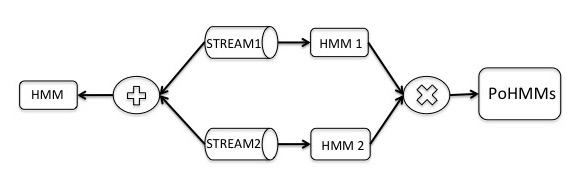
\includegraphics[width=0.6\textwidth,height=0.12\textheight]{chart.jpg}
\caption{Problem Formulation}
\label{fig:problem}
\end{figure*}

\noindent \textbf{Load Forecasting} refers to the projection of electrical load required in a certain geographical area with the use of previous electrical load usage in the same area. It is extremely important for efficient power system planning and operation, energy purchasing and generation, load switching, infrastructure development. It encompasses various factors like, historical load, weather data, population, energy supply and price, time of the year, etc.
It is usually divided into three categories, short-term forecasts (one hour to one week) , medium-term forecasts (one week to one year) and long-term forecasts (more than a year).
In short term load forecast, \cite{Bakirtzis} and \cite{Chen} used a three layer feed forward artificial neural network to predict daily load profiles. In a paper by \cite{Chow}, nonlinear autoregressive integrated neural network was used to predict daily load consumption.
In medium term load forecasts, the author forecasts \cite{Falvo} the monthly load through knowledge based activities from the output of the ANN based stage providing yearly energy predictions. Similarly, in \cite{bassi}, time lagged feedforward neural network is used to do monthly forecasting on the basis of historical series of electrical load, economic and demographic variables. Also, the authors from Covenant University, \cite{samuel} performed load forecasting of their own educational institute using the models based on linear, compound growth and cubic methods of regression analysis.
In long term load forecasting, a study done by \cite{achnata2012long} compared the performance of support vector regression and multilayer perceptron neural networks. The results showed that the percentage error in SVM reduced to 15\% when compared to neural networks trained with back propagation algorithm. It was also observed that the parameter selection in SVM plays an important role in the performance of the model.
%study done by \cite{Daneshi} resulted in showing that the models based on regression analysis did not give very accurate predictions as compared to fuzzy neural network which performed better due to better handling with non linear systems. 
Another work  \cite{Zhang} uses support vector regression to derive non linear relationship between load and economic factors like GDP for long term forecasting in developing countries.\\
Load forecasting at the utility level can be done in three ways, that are completely aggregated, completely disaggregated and by using clustering for forecasting[CITE]. In completely aggregated method, the historical consumption data is combined first and then the prediction is performed. In completely disaggregated method, first the prediction at individual level data stream is performed and then combined together to compute the overall estimate at the utility level. In case of cluster based approach, individual data streams are clustered in specific segments, then segment level consumption is predicted which is finally combined to estimate the utility level consumption. In our approach, we have historical individual level data streams that are aggregated and hence used for next day load prediction using Product of HMMs as shown in figure~\ref{fig:problem}


\noindent \textbf{Customer Segmentation} is the process of dividing a large homogeneous market into identifiable segments having similar demand characteristics. The appliance specific data has the potential to improve energy efficiency marketing by improving market segmentation, diversifying programs and transforming product development and evaluation \cite{CarrieArmel2013213}. This analysis is useful in various ways, like demand response system, intelligent distribution channel. The author \cite{wijaya2014consumer} segments the customers based on contextual dimensions like location, seasons, weather patterns, holidays, etc which help with various higher level applications like usage-specific tariff structure, theft detection, etc. In \cite{Albert}, author proposes to infer occupancy states from the consumption data by using HMM framework. They investigate the effectiveness of HMM and model based cluster analysis in producing meaningful features of the classification. 
%This work suggests the dynamics of time series as captured by HMM analysis can be valuable.

\subsection{Ensemble based learning techniques}
Ensemble learning is a method where multiple learners are trained to solve the same problem. It constructs a set of hypothesis and combines them to generate the final result.
\subsubsection{Prediction with expert advice}
A study done by \cite{Shen}, proposed a Pattern Forecasting Ensemble Model (PFEM) comprising of five forecasting models using different clustering techniques, like k-means model, self-organising map model, hierarchical clustering model, k-medoids model and fuzzy c-means model. They have showed that on three real-world dataset, their proposed ensemble model outperformed all the five individual model in case of day ahead electricity demand prediction.
Another study \cite{Felice} highlighted the importance of regularised negative correlation learning ensemble methodology on the problem of energy load hourly prediction. This method tried to overcome the problem of variability in neural network due to high sensitivitiness to the initial conditions. As this method combines the outputs of several neural networks, it achieves a marked reduction in error after introducing external data. \\
An extension of HMMs, called Factorial Hidden Markov Model (FHMM) \cite{fhmm} is a class of ensemble based learning models that addresses the need for distributed hidden states in HMMs. The FHMM generalizes the HMM by representing the state using a collection, instead of single discrete variable. However, FHMMs being directed models, when conditioned on the observed sequence, the hidden state chains become independent making the inference easy but learning more complex. Thus, the exact inference becomes intractable, leaving one to resort to approximate inference techniques like Gibbs sampling or variational approximations.


\begin{figure*}
\centering
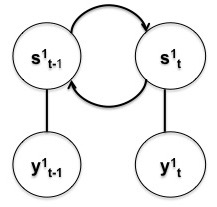
\includegraphics[width=3.3cm,height=2.6cm]{hmm1.jpg}
%\label{fig:hmm1}
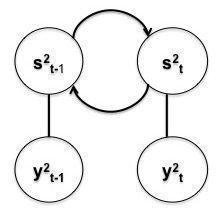
\includegraphics[width=3.3cm,height=2.6cm]{hmm2.jpg}
%\label{fig:HMMs}
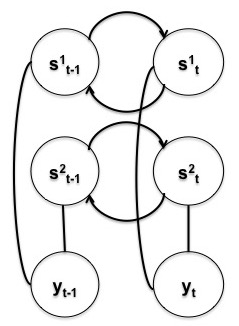
\includegraphics[width=3cm,height=3cm]{product}
\caption{HMM $S^1$ and $S^2$ and PoHMMs, P = $S^{1}$ x $S^2$}
\label{fig:HMMs}
\end{figure*}

\section{Review}
\label{sec:review}

\begin{table*}[htdp]
\begin{center}
\begin{tabular}{| c | c | c |}
\hline
Floor 0-5 & $Floor 6 -11$ & $Total$ \\
\hline
00:01:31+05:30, 786.51 & 00:01:30+05:30, 1867.34 & 00:01:29+05:30, 3369.30 \\
00:02:01+05:30, 787.24 & 00:02:00+05:30, 1850.54 & 00:01:59+05:30, 3343.39  \\
00:02:32+05:30, 787.54 & 00:02:31+05:30, 1832.85 & 00:02:30+05:30, 3339.27 \\ 
\hline
\end{tabular}
\end{center}
\caption{Timestamp readings of energy consumption for faculty housing building}
\label{table:timestamp}
\end{table*}

A Hidden Markov Model (HMM) is a statistical Markov model that represents the probability distribution over a sequence of observations \cite{Ghahramani}. They are found useful in applications like speech \cite{Rabiner}, handwriting, gesture recognition, part-of-speech tagging, bioinformatics, etc. It has two properties, first, the observation at time $t$, $y_{t}$ is generated by a process whose state at time $t$, $s_{t}$ is hidden from the observer and second, is that this hidden state process satisfies Markov property which states that given the value at state $s_{t-1}$, the value at current state $s_{t}$ is independent of all the states prior to $t-1$. The subscripts $i$ and superscripts $j$ indicate the model at $i$th time and the $j$th HMM. The state space of the HMM is discrete, that is a state can take $2$ values denoted by ON and OFF. The observed values represent the aggregated load/energy collected from different data streams at time $t$. In order to define probability distribution over the sequence of observation, it is important to define probability distribution over the initial state P($s_{1}$), the transition probability P($s_{t}|s_{t-1}$) and the observed probability P($y_{t}|s_{t}$) where $y_{t}$ is the observation at time $t$. \\
Following a notation in \cite{Rabiner}, HMM is composed of a 3-tuple \{A, B, $\pi$ \} where A is the transition probability, B is the observed probability and $\pi$ is the initial state probability.
%HMMs are widely used for modelling time series data. They are found useful in applications like speech, handwriting, gesture recognition, part-of-speech tagging, bioinformatics, etc.
HMMs solve three fundamental problems:
1. Given the model $\lambda$ = \{A, B, $\pi$ \}, and observation sequence Y = \{$y_{1}$,...,$y_{T}$\}, how do we efficiently compute the probability of the sequence of observations given the model, that is P($Y|\lambda$).
2. Given the model $\lambda$ and observation sequence Y, what is the underlying state sequence \{$s_{1}$,...,$s_{T}$\} that best explains the observations.
3. How do we adjust the model parameters (A,B,$\lambda$) so as to maximize the probability of observation sequence given the model P($Y|\lambda$). There is no optimal way to estimate the model parameters given any infinite observation sequence. However, using an iterative procedure like Baum-Welch or gradient techniques, model parameters $\lambda$ can be chosen such that P($O|\lambda$) is locally maximized. \\
In this paper, we deal with the third problem as it involves learning parameters by training the model with the past energy consumption data and then using these parameters to perform load forecasting.\\
\noindent \textbf{An Example:} Figure~\ref{fig:HMMs} shows the HMMs $S^1$ and $S^2$ generated by two data streams. The energy consumed by first six floors and the top six floors of the faculty housing building is represented by the two data streams, $S^1$ and $S^2$ individually. In order to know the energy consumption of all the 12 floors, simple addition of two data streams will not work as the readings in both the data streams are not synchronized in time. Table ~\ref{table:timestamp} shows the timestamp readings of the energy consumed by the two data streams and the entire building. As can be seen in table~\ref{table:timestamp}, the recording in both the data streams is shifted by 1 second. Also, the recording for each data stream is sampled every 30 seconds.


\subsection{Product of HMMs}
\label {pohmm}
PoHMM is a model that combines several HMMs by multiplying their individual distribution together and then renormalizing them as can be seen in equation~\ref{eq:pohmm}. Here, d is a vector in discrete space, $\theta_{m}$ is all parameters of individual model m, $f_{m}(d | \theta_{m})$ is the probability of d under model m, and c indexes all the possible vectors in the data space. Its representation includes both directed and undirected links where the hidden states are causally connected to the other hidden states but non causally related to the visible states. This causes different conditional independence relationships among the variables in graphical model. 
%It is a way of combining HMM's to form distributed state time series model. It is defined by multiplying together the densities of its, k experts and renormalizing them. 
The figure~\ref{fig:product} is a product of two HMMs P = $S^1$ x $S^2$ where the superscript in $S^1$ indicates the kth HMM. The number of states in the PoHMM is the product of states in $S^1$ and $S^2$ which is $4$ in our case. The connections formed in the P depend on the links in the multiplying HMMs. 
%The resultant HMM will have a pair (s,s) X = \{6; $R_1$$S_1$, $R_1$$S_2$, $R_1$$S_3$, $R_2$$S_1$, $R_2$$S_2$, $R_2$$S_3$\} \\
%$X_0$ = \{$R_1$$S_1$\} \\
%A = \{a,b\} \\

\begin{eqnarray}
p(d|\theta_{1}...\theta_{n}) = \frac{\prod_{m}f_m(d|\theta_{m})}{\sum_{c}\prod_{m}f_m(c|\theta_{m})}
\label{eq:pohmm}
\end{eqnarray}

\subsection{Training the model by minimising contrastive divergence}
To fit the model to the data, we need to maximize the likelihood of the dataset or minimise the Kullback-Liebler (KL) divergence between the data distribution, $P^0$ (distribution at time 0) and $P^\infty_\theta$ (also written as $p(d|\theta_{1}...\theta_{n})$) which is
the equilibrium distribution over the visible variables. KL divergence is defined as the non-symmetric measure of the difference between two probability distributions $P^\infty$ and $P^0$. It measures the information lost when $P^\infty$ is used to approximate $P^{0}$ as shown mathematically in equation~\ref{eq:KL}.

\begin{eqnarray}
P^0 || P^\infty_\theta =  \sum_{d}P^0 (d)logP^0(d) - \sum_{d}P^0 (d)logP^\infty_\theta(d)  \label{eq:KL} \\
 = \nonumber -H(P^0) - \langle log P^\infty_\theta \rangle_{P^{0}}
\end{eqnarray}

where $||$ represents KL divergence, d is the data vector in discrete space, $\theta_m$ is all the parameters of individual model m, $P^0$ is the data distribution at time $0$, $P^\infty_\theta$ (fantasy data) is the equilibrium distribution obtained after prolonged Gibbs sampling (figure~\ref{fig:gibbs}), H($P^0$) represents the entropy which is ignored during optimisation as $P^0$ does not depend on the parameters of the model, angle brackets denote the expectation over the distribution specified by the subscript. \\

 \begin{figure*}[t]
\centering
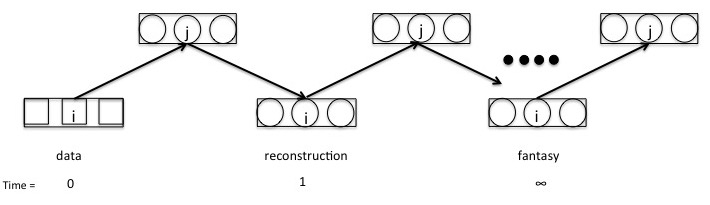
\includegraphics[width=10.5cm,height=3cm]{gibbs.jpg}
\caption{Visualization of Gibbs sampling}
\label{fig:gibbs}
\end{figure*}

In Gibbs sampling, each variable draws a sample from its posterior distribution given the current states of the other variables. The hidden states of all the models are conditionally independent given the data and hence can be parallel updated as shown in Figure~\ref{fig:gibbs}. This contributes to an important consequence of product formulation. At time t=0, the observed variables represent a data vector, d and the hidden variables, s of all the models are updated in parallel with samples from their posterior distribution given the observed variables, y. At time 1, the visible variables are updated to generate a reconstruction of the original data vector from the hidden variables and the hidden variables are again updated simultaneously. This prolonged sampling helps the Markov chain to converge to the equilibrium distribution which helps to attain the unbiased estimate of the gradient of the PoHMMs (equation~\ref{eq:gradient}) where D corresponds to the data, log$f_{\theta_{m}}$ is also be written as $f_m$($D|\theta_m$). \\

\begin{eqnarray}
 \langle \frac {\partial log P^\infty(D)} {\partial\theta_{m}} \rangle_{P^0} = \langle \frac {\partial log f_{\theta_{m}}}{\partial \theta_m} \rangle_{P^0} 
- \langle \frac {\partial log f_{\theta_{m}}}{\partial \theta_m} \rangle_{P^\infty_\theta}
\label{eq:gradient}
\end{eqnarray}

Since the samples from the equilibrium state require computation and also have high variance as they come from the entire model's distribution, it poses a difficulty in determining the estimate the derivative. Therefore, the optimisation is performed on the different objective function called contrastive divergence, defined in equation~\ref{eq:CD}. Contrastive divergence is the difference between $P^0 || P^\infty_\theta$ and $P^1_\theta || P^\infty_\theta$ where $P^1_\theta$ is the distribution over the one-step reconstruction of the data vectors generated by one full step of Gibbs sampling. The intuition behind using contrastive divergence is to leave the initial distribution $P^{0}$ over the visible variables unaltered and also the intractable expectation over $P^\infty_\theta$ gets cancelled out. Instead of comparing the initial and final derivatives, $P^0$ and $P^\infty_\theta$, the Markov chain is run for one full step and the parameters are updated to avoid the chain to wander away from the initial distribution on the first step. As $P^1$ is a step closer to $P^\infty$ which guarantees that $P^0 || P^\infty_\theta$ will always exceed $P^1_\theta || P^\infty_\theta$ ensuring a non negative value unless $P^0$ = $P^1_\theta$. If $P^0$ = $P^1_\theta$, then it implies that the chain is already in an equilibrium state, that is $P^0$ = $P^\infty_\theta$ hence making the value of contrastive divergence as $0$.

\begin{eqnarray}
- \frac {\partial} {\partial\theta_{m}} (P^0 || P^\infty_\theta - P^1_\theta || P^\infty_\theta) = \langle \frac {\partial log f_{\theta_{m}}}{\partial \theta_m} \rangle_{P^0} \label{eq:CD} \\
- \langle \frac {\partial log f_{\theta_{m}}}{\partial \theta_m} \rangle_{P^1_\theta} + \nonumber \frac{\partial{P^1_\theta}}{\partial\theta_m} \frac{\partial(P^1_\theta || P^\infty_\theta)}{\partial{P^1_\theta}}
\end{eqnarray}
In equation~\ref{eq:CD}, the first two terms on the right hand side are tractable as it is easy to sample from $P^0$ and $P^1_\theta$ but the third term represents the effect on $P^1_\theta || P^\infty_\theta$ of the change of the step reconstruction caused by the change in the $\theta_m$. Extensive simulations show that it is small and rarely differs from the result of other two terms, hence can be safely ignored. Therefore in contrastive divergence, the parameters are learned according to the equation~\ref{eq:params}.
%Also, it is possible to minimise contrastive divergence by using Markov chain that mixes very slowly, even when the one step data distribution is far from the equilibrium distribution. This can be done by using mixing techniques like weight decay that ensures every visible vector has a non zero probability given the hidden states. Weight decay works by adding an extra term to the gradient function. This extra term is the derivative of a function that penalises large weights. 
 %To minimise the contrastive divergence by using a Markov chain that slowly mixes, we can use mixing techniques like weight decay that ensures that every possible visible vector has non zero probability given the latent variables.

\begin{eqnarray}
\Delta\theta_m \propto \langle \frac {\partial log f_{\theta_{m}}}{\partial \theta_m}\rangle_{P^0} - \langle \frac {\partial log f_{\theta_{m}}}{\partial \theta_m} \rangle_{P^1_\theta} \label{eq:params}
\end{eqnarray}

%The contrastive divergence algorithm for training the PoHMM has the following steps:

%%\begin{algorithm}[H]
%% \KwData{this text}
% %\KwResult{Training of PoHMMs using contrastive divergence }
% %initialization\;
% Each model's gradient $\frac{\partial}{\partial\theta_m}$ $P(Y|\theta_m)$ (Y = $\{y_t\}_{t=1}^T$ is a visible variable) is calculated on a data point using forward backward algorithm\;
% For each model, a sample is taken from the posterior distribution of paths through state space\;
% At each time step, the distributions are multiplied and renormalized together to get the reconstruction distribution\;
% A sample from the reconstruction distribution is drawn at each time step to get a reconstructed sequence. Each model's gradient is computed on the new sequence $P(\hat Y|\theta_m)$\;
% Parameters are updated as per equation~\ref{eq:params}\;
% %\end{algorithm}
 
 \subsection{Inference in PoHMM}

The main feature of PoHMMs is its undirected graphical modelling with no direct connection among the latent variables ($S^1_{t}$ and $S^2_{t}$) as they only interact indirectly via observed variables ($Y_{t}$). The hidden variables all the experts are rendered independent when conditioned on visible variables. So, if the inference in each of the constituent model is tractable then the inference in the product is also tractable. To generate a data point in this model, all the models in PoHMMs generate an observation and if they all generated the same point then it is accepted else they again generate an observation until all the models agree to it. Therefore all the models have some influence over the generated data. So, the inference determines the the probability that all the models would have taken in order to generate the given observation. 



\section{Applications using Product of HMMs}
\label{poc}

\textbf{Aim}: In this section we demonstrate how PoHMMs can be used to model data streams and perform load forecasting. Proof-of-concepts are provided on three data sets - REDD\footnote{http://redd.csail.mit.edu/}, energy data collected from faculty housing at IIIT Delhi and Enernoc data set\footnote{http://open.enernoc.com/data/}.
%To represent streams of energy consumption data from $n$\footnote{n=2} appliances by product of $k$ HMMs.

\subsection{Data Description} 
\begin{figure*}
\centering
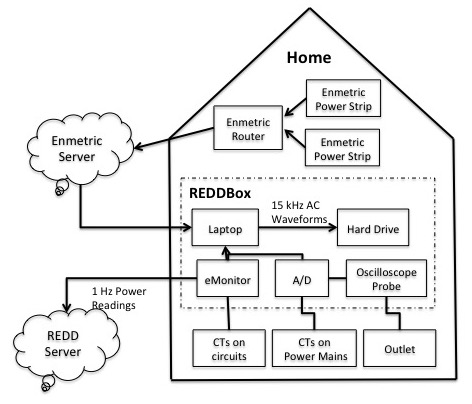
\includegraphics[width=6cm]{./REDD_img}
%\label{fig:hmm1}
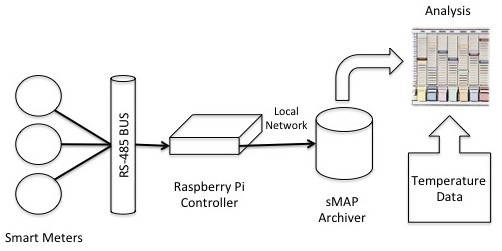
\includegraphics[width=7cm]{./FHschema}
%\label{fig:HMMs}
\caption{Schematic diagram of REDD and Faculty housing building}
\label{fig:FH}
\end{figure*}

\begin{itemize}
\item \textbf{Dataset 1:} The Reference Energy Disaggregation Data Set (REDD) contains power consumption data from real homes, for the whole house as well as for each individual circuit in
the house (labeled by the main type of appliance on that circuit). %It is intended for use in developing disaggregation methods, which can predict, from only the whole-home signal, which devices are being used.
The REDD data set contains two main types of home electricity data: high-frequency current/voltage waveform data of the two power mains (as well as the voltage signal for a single phase), and lower-frequency power data including the mains and individual, labeled circuits in the house. Its schematic diagram is shown in figure~\ref{fig:FH}.
%The main directory consists of several house directories, each of which contain all the power readings for a single house.  Each house subdirectory consists of a labels and channels files. The labels file helps in matching the channel number with the device name. Each channel file has two columns containing UTC timestamps (as integers) and power readings (recording the apparent power of the circuit) for the channel.
Experiments reported here use `house 2' data from REDD. This dataset has $318759$ records and $2$ columns. We randomly sample $300$ records for our initial experiment.
%The time series data of the microwave, dryer, kitchen$\_2$ and refrigerator are plotted below in Figures~\ref{fig:micro}, ~\ref{fig:washer}, ~\ref{fig:kitchen2}, ~\ref{fig:refri}. 

\item \textbf{Dataset 2:} This data represents the energy consumed by the IIIT Delhi's Faculty Housing (FH) building. As a part of research, a team from the institute has installed various temperature, light and motion sensors to perform real world studies and to analyse user preferences for energy conservation. Its schematic diagram is shown in figure~\ref{fig:FH}. For our analysis, we selected $1$ month's historical data ranging from 01-01-2014, 00:01 hours to 31-01-2014, 23:59 hours. The two smart meters installed, captured data from all the $12$ floors. The first meter records readings from ground to $5$th floor generating one stream of data and the second meter generates a stream from $6$th to $11$th. Both these streams are aggregated to obtain the aggregated load of the housing building. The dataset includes timestamp and power consumed in watts. There are $84133$ records in this dataset. We also have the total energy consumed by the faculty housing building which would serve as the ground truth to compare the aggregated load using PoHMMs. 

\item \textbf{Dataset 3:} The third dataset that we have used is the Enernoc data set, which consists of power consumption data from different industrial customers. This contains energy consumption data of 100 industrial consumers from January 2012 to December 2012. In our analysis, we have used 66\% of data for training and 33\% for testing. We are comparing the load forecast by using PoHMMs vs single HMM. The metric used to measure the difference between the distribution of both the methods is KL divergence (refer equation\ref{eq:KL}). Hence, lesser value of KL divergence would mean more similar distributions. The comparisons using both the above approaches are done to observe the behaviour at different time scales, number of consumers and type of consumers.
\end{itemize}


\subsection{Problem Formulation}
The disparate energy data streams collects readings at different time scales. Each of the data stream is modelled as a HMM/ expert with cardinality $2$, that is either ON or OFF. The process of aggregating the energy data from different data streams is modelled through PoHMMs. 

%Different smart meters can send data points when they are collected resulting in inconsistent data including aggregating non-aligned time stamped readings, readings with missing values, repeated values, meter reset readings.
%We address the problem of learning from disparate data streams (with inconsistencies) by modelling streams as HMMs and the process of aggregating data at the base station as a Product of HMMs. This enables us to perform load forecasting using machine learning techniques.
Each energy data stream is used to train the model, till the time the objective function, that is contrastive divergence reaches a threshold value. Once the model is trained from a randomly sampled data stream, the parameters learned by the model %(mixing component of each unigauss, means of gaussian bits, log precisions of axis-aligned gaussian bits) 
are provided to the randomly sampled test set (total energy consumed data) to obtain the conditional probability distribution of the gaussians given the data. Similarly, all the data streams are used for training the model, and the parameters learned are then applied on the test set to obtain the conditional probability of the gaussians given the data. After all the data streams are used to obtain the probability distribution, we use the data stream that correspond to the total energy consumed from the house/ building to train the model and hence obtain the probability distribution P of the gaussians. These probability distributions are then compared with the product of the probability distributions Q obtained from the individual data streams. The evaluation of how well the learning has taken place is done by using a KL divergence. KL divergence of two probability distributions P and Q, $D_{KL}$(P$\parallel$Q) is the measure of information lost when Q is used to approximate P. Figure~\ref{fig:problem} shows a flowchart that depicts the problem formulation.
%Here, P is the real data and Q is a fantasy data. The two probability distributions in the REDD example refer to the expert probabilities in real and fantasy data. 
%The learned parameters from the training are fitted to the fantasy data to measure the information lost when fantasy data is used to approximate real data.

\subsubsection{Implementation Details}
The implementation of the product of hidden Markov model is obtained from Iain Murray's website\footnote{\label{link}http://homepages.inf.ed.ac.uk/imurray2/code/}. It implements the technique described in paper \cite{hinton2000}.

%\begin{table*}[htdp]
%\parbox{.39\linewidth}{
%\centering
%\begin{tabular}{| c | c | c | c |}
%\hline
%Samples & $KL Div$ & $Iterations$& $T(sec)$ \\
%\hline
%300 & 2.4864 & 18600 & 186.212 $\pm$9.087  \\
%500 & 0.6761 & 10200 & 106.564 $\pm$10.046 \\
%1000 & 1.1088 & 11200 & 158.521 $\pm$1.97  \\
%1500 & 3.8829 & 5300 & 92.896 $\pm$8.075  \\
%2000 & 1.8686 & 6900 & 130.98 $\pm$1.932 \\
%2500 & 0.4733 & 9900 & 215.563 $\pm$ 2.471 \\
%3000 & 2.8204 & 11000 & 258.213 $\pm1.918$ \\
%3500 & 1.2332 & 7900 & 204.661 $\pm$1.713 \\
%4000 & 0.8959 & 10400 & 292.666 $\pm$0.619 \\
%4500 & 1.1118 & 7200 & 222.558 $\pm$1.967 \\
%8000 & 6.392 & 8100 & 381.635 $\pm$2.952  \\
%10000 & 8.276 & 10500 & 887.932 $\pm$13.824  \\
%15000 & 0.7201 & 9400 & 1368.514 $\pm$13.605  \\
%\hline
%\end{tabular}
%\caption{Effect of varying samples (REDD)}
%\label{table:sample1}}
%\hfill
%\parbox{.65\linewidth}{
%\centering
%\begin{tabular}{| c | c | c | c |}
%\hline
%Samples & $KL Div$  & $Iterations$ & $T(sec)$\\
%\hline
%100 & 0.26219 & 45100 & 257  \\
%300 & 0.19753 & 43200 & 222 \\
%500 & 0.55493 & 44800 & 260  \\
%700 & 0.32847 & 44000 & 249 \\
%900 & 3.9486 & 42600 & 221  \\
%1100 & 4.9274 & 44700 & 317  \\
%1300 & 3.0425 & 43100 & 276 \\
%1500 &  3.1128 & 44400 & 303 \\
%2000 & 1.9192 & 44400 & 306 \\
%2500 & 1.7122 & 44100 & 370 \\
%3000 & 1.4686 & 43300 & 331 \\
%3500 & 1.2663 & 43200 & 370  \\
%4000 & 1.0793 & 43200 & 403  \\
%\hline
%\end{tabular}
%\caption{Effect of varying samples (housing data), KL Div in e-04}
%\label{table:sample2}}
%\end{table*}
%
%\begin{table*}[htdp]
%\parbox{.4\linewidth}{
%\centering
%\begin{tabular}{| c | c | c | c | c | c |}
%\hline
%Samples & $T_{P}$ & $T_H$ & $Iter_P$ & $Iter_H$ & $KL Div $\\
%\hline
%600 & 92 & 91 & 8000 & 26900 & 20.82 \\
%1500 & 127 & 130 & 5700 & 15300 & 11.14  \\
%1800 & 180 & 166 & 5900 & 15100 & 12.59 \\
%2500 & 485 & 127 & 5800 & 5500 & 6.87 \\
%\hline
%\end{tabular}
%\caption{Effect of varying samples (Enernoc)}
%\label{table:sample3}}
%\hfill
%\parbox{.65\linewidth}{
%\centering
%\begin{tabular}{| c | c | c | c | c | c |}
%\hline
%Experts & $T_P$ & $T_H$ & $Iter_P$& $Iter_H$ & $KL Div $\\
%\hline
%3 & 102 & 463 & 14100 & 210200 & 4.09 \\
%5 & 49 & 79 & 6300 & 27700 & 13.75  \\
%7 & 80 & 44 & 8600 & 14500 & 7.46 \\
%10 & 66 & 60 & 6100 & 16600 & 4.355  \\
%15 & 113 & 127 & 8200 & 27500 & 6  \\
%\hline
%\end{tabular}
%\caption{Effect of varying HMMs (Enernoc)}
%\label{table:expert2}}
%\end{table*}

\begin{figure*}
\centering
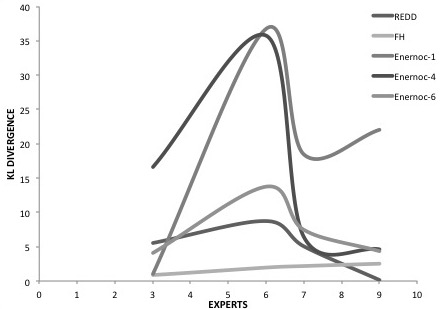
\includegraphics[width=7cm]{./plot4.jpg}
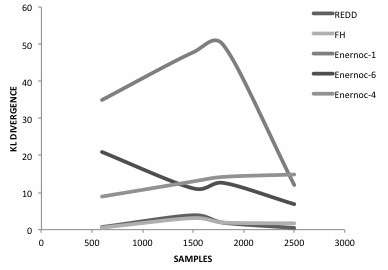
\includegraphics[width=7cm]{./plot5.jpg}
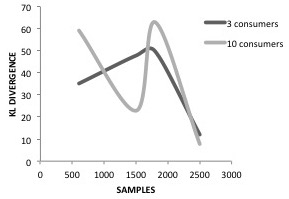
\includegraphics[width=7cm]{./plot3.jpg}
\caption{Comparison of REDD, FH and Enernoc data sets}
\label{fig:plots}
\end{figure*}


\subsection{Empirical Results}
All the experiments were performed on two machines, a personal machine with 8GB Ram, Intel Core i7 CPU @ 2.9GHz and a HPC server with 20 CPUs @ 2.5GHz, 10 cores/socket, 2 sockets and 99 GB RAM.  
%In case of REDD, Tables~\ref{table:sample1},~\ref{table:threshold1} and \ref{table:expert1} show the effect of varying data samples, threshold and no. of experts on KL divergence. 
Figure~\ref{fig:plots} shows three plots, first two show the relationship of KL Divergence with varying number of experts and samples respectively. This comparison is done between REDD, FH, Enernoc-1 (1 month data), Enernoc-4 and Enernoc-6. As seen in the first plot of figure~\ref{fig:plots}, (Enernoc-1 and Enernoc-4) and (Enernoc-6 and REDD) follow a similar trend. Amongst all the datasets, REDD attains the minimum KL divergence followed by FH. FH dataset has minimum deviation amongst the rest of the datasets. Similarly, in the second plot we can observe that FH and REDD attain the minimum divergence when varied across the different data samples. Thus our experiments show that the divergence in aggregate forecasting is less in residential dataset as compared to industrial dataset.\\

The detailed empirical results are shown in Appendix~\ref{App:AppendixA}. 
%The data samples are randomly selected from the dataset, KL divergence is chosen as the performance metric, iterations are performed to obtain the samples from the equilibrium distribution by using Gibbs sampler on the hidden and visible variables and the average time (in seconds) taken with the standard deviation on three such iterations is noted.
%
%In case of faculty housing dataset, Tables~\ref{table:sample2},~\ref{table:threshold2} and \ref{table:expert2} show the effect of varying data samples, threshold and no. of HMMs on the KL divergence.
%As per table \ref{table:sample1} and \ref{table:sample2}, there is no linear relationship between no. of samples and KL divergence. 
%%The best performance was attained when $2500$ and $300$ samples were randomly chosen from the REDD and faculty housing dataset respectively. 
%In table \ref{table:threshold1} and \ref{table:threshold2}, there is an indirect relationship between threshold and KL divergence value, that is lower the threshold, higher the KL divergence. 
%%Similarly, the relationship between threshold values and iterations/time taken is indirect.
%In table \ref{table:expert1} and \ref{table:expert2}, it can be seen that the KL divergence attains its minimum value when the no. of HMMs multiplied are same as the number of data streams aggregated. Hence, the error is minimum when the number of HMMs reaches the number of aggregated data streams, that is when all the appliances in `house 2' (total appliances are $9$) of REDD are used in PoHMMs and when both the data streams of faculty housing building are aggregated together.
%Figure~\ref{fig:plot} shows how KL Divergence behaves with varying data samples and experts for 1 month, 4 months and 6 months data. We can see that the curve representing KL divergence (6 months) stays lower than the rest through out the time period. Also, we can see that the curves attain their minimum values when more number data samples are used for training and testing.

%\begin{table*}[htdp]
%\parbox{.39\linewidth}{
%\centering
%\begin{tabular}{| c | c | c | c |}
%\hline
%Threshold & $KL Div$ & $Iterations$ & $T(sec)$  \\
%\hline
%.1 & 0.473 & 9900 & 210.6 $\pm$1.493 \\
%.05 & 0.443 & 10900 & 240.607$\pm$2.436 \\
%.01 & 0.454 & 18000 & 431.536 $\pm$14.509 \\
%.005 & 0.509 & 49800 & 1167.243 $\pm$43.412 \\
%\hline
%\end{tabular}
%\caption{Effect of varying threshold (REDD)}
%\label{table:threshold1}
%}
%\hfill
%\parbox{.65\linewidth}{
%\centering
%\begin{tabular}{| c | c | c | c |}
%\hline
%Threshold & $KL Div$ & $Iterations$& $T(sec)$ \\
%\hline
%0.9 & 0.768 & 49300 & 153.67 $\pm$13.57  \\
%0.8 & 0.768 & 49300 & 190.3 $\pm$34.35 \\
%0.7 & 0.769 & 49400 &  193.67$\pm$31.64  \\
%0.6 & 0.792 & 49500 & 218.3 $\pm$43.93  \\
%0.5 & 0.793 & 49600 & 250.67$\pm$3.51  \\
%0.4 & 0.854 & 49600 & 191$\pm$35.55  \\
%\hline
%\end{tabular}
%\caption{Effect of varying threshold (housing data), KL Div in e-04}
%\label{table:threshold2}
%}
%\end{table*}
%
%\begin{table*}[htdp]
%\parbox{.39\linewidth}{
%\centering
%\begin{tabular}{| c | c | c | c |}
%\hline
%Experts & $KL Div$ & $Iterations$ & $T(sec)$  \\
%\hline
%3 & 5.559  & 10700 & 233.664 $\pm$0.579 \\
%4 & 0.188 & 19900 & 465.634 $\pm$5.275  \\
%5 & 0.432  & 13400 & 338.416 $\pm$3.988  \\
%6 & 8.736  & 28100 & 606.062 $\pm$7.534 \\
%7 & 5.054  & 17300 & 411.457 $\pm$10.051\\
%8 & 0.436 & 10700 & 260.544 $\pm$27.862 \\
%9 & 0.15 & 20600 & 474.579 $\pm$14.619 \\
%\hline
%\end{tabular}
%\caption{Effect of varying experts (REDD)}
%\label{table:expert1}}
%\hfill
%\parbox{.65\linewidth}{
%\centering
%\begin{tabular}{| c | c | c | c |}
%\hline
%Experts & $KL Div$ & Iterations & $T(sec)$\\
%\hline
%2 & 0 & 49200 & 233.33 $\pm$7.23 \\
%3 & 0.81 & 49200 & 237.67 $\pm$10.59 \\
%5 & 0.77 & 49300 & 242.33 $\pm$3 \\
%10 & 2.12 & 49300 & 228.33 $\pm$46.23 \\
%15 & 2.55 & 49300 & 269.33 $\pm$17.61 \\
%20 & 2.23 & 49300 & 305.66 $\pm$2.08  \\
%25 & 2.19 & 49300 & 302.33 $\pm$8 \\
%30 & 2.24 & 49300 & 336.33 $\pm$9.5 \\
%35 & 1.94 & 49300 & 331.33 $\pm$9 \\
%\hline
%\end{tabular}
%\caption{Effect of varying experts (housing data), KL Div in e-04}
%\label{table:expert2}
%}
%\end{table*}


\section{Conclusion}
\label{conclusion}

In this paper, we are solving the problem of load aggregation (energy consumption) and aggregate forecasting for disparate energy data sources using the ensemble based learning technique called Product of HMMs. Several challenges are faced while computing the aggregated energy, few of which include non-aligned timestamp readings, missing values, meter reset readings. This technique produces the combined probability distributions of several simpler distributions and then renormalizes the output. The optimization problem is to minimize the contrastive divergence between the two probability distributions of the data at time $0$ and the data at time $1$ (one-step reconstruction using Gibbs sampling). The evaluation of the algorithm is done by computing the KL divergence between the product of the energy data distributions and the total energy data distribution.
 From the results shown in table \ref{table:expert1} and \ref{table:expert2}, we can see that the algorithm has performed best when the number of appliances (REDD) reached the actual number of appliances ($9$) in the house and the number of data streams in case of FH data reached the actual number of streams ($2$) used in the 12 floor building. Therefore, this signifies that this algorithm is applicable for this kind of application and can be used for load forecasting.


\section*{Acknowledgment}
The authors would like to thank $EMC^2$ for supporting this research through grant number JRA092014-Q3-5.
%
%
%The authors would like to thank...

\nocite{Zoha12articlenon-intrusive,CarrieArmel2013213,eps272990,NIPS2010,Rabiner,SS97a,Kawamoto,Diane,Klopfert,Ghahramani,Felice,Shen,taban,Albert,wijaya2014consumer,Zhang,achnata2012long,bassi,samuel,Falvo,Bakirtzis,Chen,Chow,DisaggregationHSMM,KolterJ12,KolterF11,BLTJ:BLTJ21650,Heinzelman00energy,Taylor,NYAS:NYAS5921,
Wijaya,5620917,1626400,mckerracher,hinton2000,aistats,fhmm,andrew}



%\section{The {\secit Body} of The Paper}
%Typically, the body of a paper is organized
%into a hierarchical structure, with numbered or unnumbered
%headings for sections, subsections, sub-subsections, and even
%smaller sections.  The command \texttt{{\char'134}section} that
%precedes this paragraph is part of such a
%hierarchy.\footnote{This is the second footnote.  It
%starts a series of three footnotes that add nothing
%informational, but just give an idea of how footnotes work
%and look. It is a wordy one, just so you see
%how a longish one plays out.} \LaTeX\ handles the numbering
%and placement of these headings for you, when you use
%the appropriate heading commands around the titles
%of the headings.  If you want a sub-subsection or
%smaller part to be unnumbered in your output, simply append an
%asterisk to the command name.  Examples of both
%numbered and unnumbered headings will appear throughout the
%balance of this sample document.
%
%Because the entire article is contained in
%the \textbf{document} environment, you can indicate the
%start of a new paragraph with a blank line in your
%input file; that is why this sentence forms a separate paragraph.
%
%\subsection{Type Changes and {\subsecit Special} Characters}
%We have already seen several typeface changes in this sample.  You
%can indicate italicized words or phrases in your text with
%the command \texttt{{\char'134}textit}; emboldening with the
%command \texttt{{\char'134}textbf}
%and typewriter-style (for instance, for computer code) with
%\texttt{{\char'134}texttt}.  But remember, you do not
%have to indicate typestyle changes when such changes are
%part of the \textit{structural} elements of your
%article; for instance, the heading of this subsection will
%be in a sans serif\footnote{A third footnote, here.
%Let's make this a rather short one to
%see how it looks.} typeface, but that is handled by the
%document class file. Take care with the use
%of\footnote{A fourth, and last, footnote.}
%the curly braces in typeface changes; they mark
%the beginning and end of
%the text that is to be in the different typeface.
%
%You can use whatever symbols, accented characters, or
%non-English characters you need anywhere in your document;
%you can find a complete list of what is
%available in the \textit{\LaTeX\
%User's Guide}\cite{Lamport:LaTeX}.
%
%\subsection{Math Equations}
%You may want to display math equations in three distinct styles:
%inline, numbered or non-numbered display.  Each of
%the three are discussed in the next sections.
%
%\subsubsection{Inline (In-text) Equations}
%A formula that appears in the running text is called an
%inline or in-text formula.  It is produced by the
%\textbf{math} environment, which can be
%invoked with the usual \texttt{{\char'134}begin. . .{\char'134}end}
%construction or with the short form \texttt{\$. . .\$}. You
%can use any of the symbols and structures,
%from $\alpha$ to $\omega$, available in
%\LaTeX\cite{Lamport:LaTeX}; this section will simply show a
%few examples of in-text equations in context. Notice how
%this equation: \begin{math}\lim_{n\rightarrow \infty}x=0\end{math},
%set here in in-line math style, looks slightly different when
%set in display style.  (See next section).
%
%\subsubsection{Display Equations}
%A numbered display equation -- one set off by vertical space
%from the text and centered horizontally -- is produced
%by the \textbf{equation} environment. An unnumbered display
%equation is produced by the \textbf{displaymath} environment.
%
%Again, in either environment, you can use any of the symbols
%and structures available in \LaTeX; this section will just
%give a couple of examples of display equations in context.
%First, consider the equation, shown as an inline equation above:
%\begin{equation}\lim_{n\rightarrow \infty}x=0\end{equation}
%Notice how it is formatted somewhat differently in
%the \textbf{displaymath}
%environment.  Now, we'll enter an unnumbered equation:
%\begin{displaymath}\sum_{i=0}^{\infty} x + 1\end{displaymath}
%and follow it with another numbered equation:
%\begin{equation}\sum_{i=0}^{\infty}x_i=\int_{0}^{\pi+2} f\end{equation}
%just to demonstrate \LaTeX's able handling of numbering.
%
%\subsection{Citations}
%Citations to articles \cite{bowman:reasoning, clark:pct, braams:babel, herlihy:methodology},
%conference
%proceedings \cite{clark:pct} or books \cite{salas:calculus, Lamport:LaTeX} listed
%in the Bibliography section of your
%article will occur throughout the text of your article.
%You should use BibTeX to automatically produce this bibliography;
%you simply need to insert one of several citation commands with
%a key of the item cited in the proper location in
%the \texttt{.tex} file \cite{Lamport:LaTeX}.
%The key is a short reference you invent to uniquely
%identify each work; in this sample document, the key is
%the first author's surname and a
%word from the title.  This identifying key is included
%with each item in the \texttt{.bib} file for your article.
%
%The details of the construction of the \texttt{.bib} file
%are beyond the scope of this sample document, but more
%information can be found in the \textit{Author's Guide},
%and exhaustive details in the \textit{\LaTeX\ User's
%Guide}\cite{Lamport:LaTeX}.
%
%This article shows only the plainest form
%of the citation command, using \texttt{{\char'134}cite}.
%This is what is stipulated in the SIGS style specifications.
%No other citation format is endorsed.
%
%\subsection{Tables}
%Because tables cannot be split across pages, the best
%placement for them is typically the top of the page
%nearest their initial cite.  To
%ensure this proper ``floating'' placement of tables, use the
%environment \textbf{table} to enclose the table's contents and
%the table caption.  The contents of the table itself must go
%in the \textbf{tabular} environment, to
%be aligned properly in rows and columns, with the desired
%horizontal and vertical rules.  Again, detailed instructions
%on \textbf{tabular} material
%is found in the \textit{\LaTeX\ User's Guide}.
%
%Immediately following this sentence is the point at which
%Table 1 is included in the input file; compare the
%placement of the table here with the table in the printed
%dvi output of this document.
%
%\begin{table}
%\centering
%\caption{Frequency of Special Characters}
%\begin{tabular}{|c|c|l|} \hline
%Non-English or Math&Frequency&Comments\\ \hline
%\O & 1 in 1,000& For Swedish names\\ \hline
%$\pi$ & 1 in 5& Common in math\\ \hline
%\$ & 4 in 5 & Used in business\\ \hline
%$\Psi^2_1$ & 1 in 40,000& Unexplained usage\\
%\hline\end{tabular}
%\end{table}
%
%To set a wider table, which takes up the whole width of
%the page's live area, use the environment
%\textbf{table*} to enclose the table's contents and
%the table caption.  As with a single-column table, this wide
%table will ``float" to a location deemed more desirable.
%Immediately following this sentence is the point at which
%Table 2 is included in the input file; again, it is
%instructive to compare the placement of the
%table here with the table in the printed dvi
%output of this document.
%
%
%\begin{table*}
%\centering
%\caption{Some Typical Commands}
%\begin{tabular}{|c|c|l|} \hline
%Command&A Number&Comments\\ \hline
%\texttt{{\char'134}alignauthor} & 100& Author alignment\\ \hline
%\texttt{{\char'134}numberofauthors}& 200& Author enumeration\\ \hline
%\texttt{{\char'134}table}& 300 & For tables\\ \hline
%\texttt{{\char'134}table*}& 400& For wider tables\\ \hline\end{tabular}
%\end{table*}
%% end the environment with {table*}, NOTE not {table}!
%
%\subsection{Figures}
%Like tables, figures cannot be split across pages; the
%best placement for them
%is typically the top or the bottom of the page nearest
%their initial cite.  To ensure this proper ``floating'' placement
%of figures, use the environment
%\textbf{figure} to enclose the figure and its caption.
%
%This sample document contains examples of \textbf{.eps}
%and \textbf{.ps} files to be displayable with \LaTeX.  More
%details on each of these is found in the \textit{Author's Guide}.
%
%%\begin{figure}
%%\centering
%%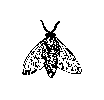
\epsfig{file=fly.eps}
%%\caption{A sample black and white graphic (.eps format).}
%%\end{figure}
%%
%%\begin{figure}
%%\centering
%%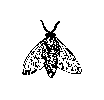
\epsfig{file=fly.eps, height=1in, width=1in}
%%\caption{A sample black and white graphic (.eps format)
%%that has been resized with the \texttt{epsfig} command.}
%%\end{figure}
%
%
%As was the case with tables, you may want a figure
%that spans two columns.  To do this, and still to
%ensure proper ``floating'' placement of tables, use the environment
%\textbf{figure*} to enclose the figure and its caption.
%
%Note that either {\textbf{.ps}} or {\textbf{.eps}} formats are
%used; use
%the \texttt{{\char'134}epsfig} or \texttt{{\char'134}psfig}
%commands as appropriate for the different file types.
%
%\subsection{Theorem-like Constructs}
%Other common constructs that may occur in your article are
%the forms for logical constructs like theorems, axioms,
%corollaries and proofs.  There are
%two forms, one produced by the
%command \texttt{{\char'134}newtheorem} and the
%other by the command \texttt{{\char'134}newdef}; perhaps
%the clearest and easiest way to distinguish them is
%to compare the two in the output of this sample document:
%
%This uses the \textbf{theorem} environment, created by
%the\linebreak\texttt{{\char'134}newtheorem} command:
%\newtheorem{theorem}{Theorem}
%\begin{theorem}
%Let $f$ be continuous on $[a,b]$.  If $G$ is
%an antiderivative for $f$ on $[a,b]$, then
%\begin{displaymath}\int^b_af(t)dt = G(b) - G(a).\end{displaymath}
%\end{theorem}
%
%The other uses the \textbf{definition} environment, created
%by the \texttt{{\char'134}newdef} command:
%\newdef{definition}{Definition}
%\begin{definition}
%If $z$ is irrational, then by $e^z$ we mean the
%unique number which has
%logarithm $z$: \begin{displaymath}{\log e^z = z}\end{displaymath}
%\end{definition}
%
%%\begin{figure}
%%\centering
%%\psfig{file=rosette.ps, height=1in, width=1in,}
%%\caption{A sample black and white graphic (.ps format) that has
%%been resized with the \texttt{psfig} command.}
%%\end{figure}
%
%Two lists of constructs that use one of these
%forms is given in the
%\textit{Author's  Guidelines}.
%
%%\begin{figure*}
%%\centering
%%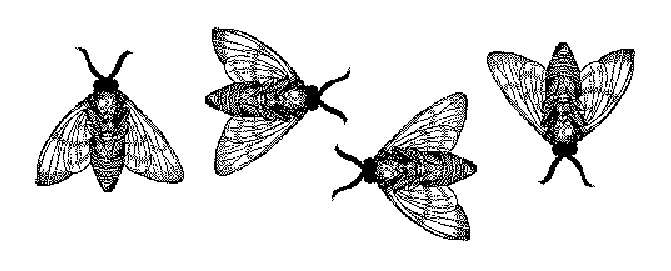
\epsfig{file=flies.eps}
%%\caption{A sample black and white graphic (.eps format)
%%that needs to span two columns of text.}
%%\end{figure*}
%and don't forget to end the environment with
%{figure*}, not {figure}!
% 
%There is one other similar construct environment, which is
%already set up
%for you; i.e. you must \textit{not} use
%a \texttt{{\char'134}newdef} command to
%create it: the \textbf{proof} environment.  Here
%is a example of its use:
%\begin{proof}
%Suppose on the contrary there exists a real number $L$ such that
%\begin{displaymath}
%\lim_{x\rightarrow\infty} \frac{f(x)}{g(x)} = L.
%\end{displaymath}
%Then
%\begin{displaymath}
%l=\lim_{x\rightarrow c} f(x)
%= \lim_{x\rightarrow c}
%\left[ g{x} \cdot \frac{f(x)}{g(x)} \right ]
%= \lim_{x\rightarrow c} g(x) \cdot \lim_{x\rightarrow c}
%\frac{f(x)}{g(x)} = 0\cdot L = 0,
%\end{displaymath}
%which contradicts our assumption that $l\neq 0$.
%\end{proof}
%
%Complete rules about using these environments and using the
%two different creation commands are in the
%\textit{Author's Guide}; please consult it for more
%detailed instructions.  If you need to use another construct,
%not listed therein, which you want to have the same
%formatting as the Theorem
%or the Definition\cite{salas:calculus} shown above,
%use the \texttt{{\char'134}newtheorem} or the
%\texttt{{\char'134}newdef} command,
%respectively, to create it.
%
%\subsection*{A {\secit Caveat} for the \TeX\ Expert}
%Because you have just been given permission to
%use the \texttt{{\char'134}newdef} command to create a
%new form, you might think you can
%use \TeX's \texttt{{\char'134}def} to create a
%new command: \textit{Please refrain from doing this!}
%Remember that your \LaTeX\ source code is primarily intended
%to create camera-ready copy, but may be converted
%to other forms -- e.g. HTML. If you inadvertently omit
%some or all of the \texttt{{\char'134}def}s recompilation will
%be, to say the least, problematic.
%
%\section{Conclusions}
%This paragraph will end the body of this sample document.
%Remember that you might still have Acknowledgments or
%Appendices; brief samples of these
%follow.  There is still the Bibliography to deal with; and
%we will make a disclaimer about that here: with the exception
%of the reference to the \LaTeX\ book, the citations in
%this paper are to articles which have nothing to
%do with the present subject and are used as
%examples only.
%%\end{document}  % This is where a 'short' article might terminate
%
%%ACKNOWLEDGMENTS are optional
%\section{Acknowledgments}
%This section is optional; it is a location for you
%to acknowledge grants, funding, editing assistance and
%what have you.  In the present case, for example, the
%authors would like to thank Gerald Murray of ACM for
%his help in codifying this \textit{Author's Guide}
%and the \textbf{.cls} and \textbf{.tex} files that it describes.
%



%
% The following two commands are all you need in the
% initial runs of your .tex file to
% produce the bibliography for the citations in your paper.
\bibliographystyle{abbrv}
\bibliography{sigproc-sp}  % sigproc.bib is the name of the Bibliography in this case
% You must have a proper ".bib" file
%  and remember to run:
% latex bibtex latex latex
% to resolve all references
%
% ACM needs 'a single self-contained file'!
%
%APPENDICES are optional
%\balancecolumns
\newpage
\appendix
\section{Empirical Results} 
\label{App:AppendixA}

The data samples are randomly selected from the dataset, KL divergence is chosen as the performance metric, iterations are performed to obtain the samples from the equilibrium distribution by using Gibbs sampler on the hidden and visible variables and the average time (in seconds) taken with the standard deviation on three such iterations is noted.

In case of faculty housing dataset, Tables~\ref{table:sample2},~\ref{table:threshold2} and \ref{table:expert2} show the effect of varying data samples, threshold and no. of HMMs on the KL divergence.
As per table \ref{table:sample1} and \ref{table:sample2}, there is no linear relationship between no. of samples and KL divergence. 
%The best performance was attained when $2500$ and $300$ samples were randomly chosen from the REDD and faculty housing dataset respectively. 
In table \ref{table:threshold1} and \ref{table:threshold2}, there is an indirect relationship between threshold and KL divergence value, that is lower the threshold, higher the KL divergence. 
%Similarly, the relationship between threshold values and iterations/time taken is indirect.

In table \ref{table:expert1} and \ref{table:expert2}, it can be seen that the KL divergence attains its minimum value when the no. of HMMs multiplied are same as the number of data streams aggregated. Hence, the error is minimum 
when the number of HMMs reaches the number of aggregated data streams, that is when all the appliances in `house 2' (total appliances are $9$) of REDD are used in PoHMMs and when both the data streams of faculty housing building are aggregated together.

%Figure~\ref{fig:plot} shows how KL divergence behaves with varying data samples and experts for 1 month, 4 months and 6 months data. We can see that the curve representing KL divergence (6 months) stays lower than the rest through out the time period. Also, we can see that the curves attain their minimum values when more number data samples are used for training and testing.

\begin{table*}[htdp]
\parbox{.39\linewidth}{
\centering
\begin{tabular}{| c | c | c | c |}
\hline
Samples & $KL Div$ & $Iterations$& $T(sec)$ \\
\hline
300 & 2.4864 & 18600 & 186.212 $\pm$9.087  \\
500 & 0.6761 & 10200 & 106.564 $\pm$10.046 \\
1000 & 1.1088 & 11200 & 158.521 $\pm$1.97  \\
1500 & 3.8829 & 5300 & 92.896 $\pm$8.075  \\
2000 & 1.8686 & 6900 & 130.98 $\pm$1.932 \\
2500 & 0.4733 & 9900 & 215.563 $\pm$ 2.471 \\
3000 & 2.8204 & 11000 & 258.213 $\pm1.918$ \\
3500 & 1.2332 & 7900 & 204.661 $\pm$1.713 \\
4000 & 0.8959 & 10400 & 292.666 $\pm$0.619 \\
4500 & 1.1118 & 7200 & 222.558 $\pm$1.967 \\
8000 & 6.392 & 8100 & 381.635 $\pm$2.952  \\
10000 & 8.276 & 10500 & 887.932 $\pm$13.824  \\
15000 & 0.7201 & 9400 & 1368.514 $\pm$13.605  \\
\hline
\end{tabular}
\caption{Effect of varying samples (REDD)}
\label{table:sample1}}
\hfill
\parbox{.65\linewidth}{
\centering
\begin{tabular}{| c | c | c | c |}
\hline
Samples & $KL Div$  & $Iterations$ & $T(sec)$\\
\hline
100 & 0.26219 & 45100 & 257  \\
300 & 0.19753 & 43200 & 222 \\
500 & 0.55493 & 44800 & 260  \\
700 & 0.32847 & 44000 & 249 \\
900 & 3.9486 & 42600 & 221  \\
1100 & 4.9274 & 44700 & 317  \\
1300 & 3.0425 & 43100 & 276 \\
1500 &  3.1128 & 44400 & 303 \\
2000 & 1.9192 & 44400 & 306 \\
2500 & 1.7122 & 44100 & 370 \\
3000 & 1.4686 & 43300 & 331 \\
3500 & 1.2663 & 43200 & 370  \\
4000 & 1.0793 & 43200 & 403  \\
\hline
\end{tabular}
\caption{Effect of varying samples (housing data), KL Div in e-04}
\label{table:sample2}}
\end{table*}

\begin{table*}[htdp]
\parbox{.4\linewidth}{
\centering
\begin{tabular}{| c | c | c | c | c | c |}
\hline
Samples & $T_{P}$ & $T_H$ & $Iter_P$ & $Iter_H$ & $KL Div $\\
\hline
600 & 92 & 91 & 8000 & 26900 & 20.82 \\
1500 & 127 & 130 & 5700 & 15300 & 11.14  \\
1800 & 180 & 166 & 5900 & 15100 & 12.59 \\
2500 & 485 & 127 & 5800 & 5500 & 6.87 \\
\hline
\end{tabular}
\caption{Effect of varying samples (Enernoc-6)}
\label{table:sample3}}
\hfill
\parbox{.65\linewidth}{
\centering
\begin{tabular}{| c | c | c | c | c | c |}
\hline
Experts & $T_P$ & $T_H$ & $Iter_P$& $Iter_H$ & $KL Div $\\
\hline
3 & 102 & 463 & 14100 & 210200 & 4.09 \\
5 & 49 & 79 & 6300 & 27700 & 13.75  \\
7 & 80 & 44 & 8600 & 14500 & 7.46 \\
10 & 66 & 60 & 6100 & 16600 & 4.355  \\
15 & 113 & 127 & 8200 & 27500 & 6  \\
\hline
\end{tabular}
\caption{Effect of varying HMMs (Enernoc-6)}
\label{table:expert2}}
\end{table*}

\begin{table*}[htdp]
\parbox{.39\linewidth}{
\centering
\begin{tabular}{| c | c | c | c |}
\hline
Threshold & $KL Div$ & $Iterations$ & $T(sec)$  \\
\hline
.1 & 0.473 & 9900 & 210.6 $\pm$1.493 \\
.05 & 0.443 & 10900 & 240.607$\pm$2.436 \\
.01 & 0.454 & 18000 & 431.536 $\pm$14.509 \\
.005 & 0.509 & 49800 & 1167.243 $\pm$43.412 \\
\hline
\end{tabular}
\caption{Effect of varying threshold (REDD)}
\label{table:threshold1}
}
\hfill
\parbox{.65\linewidth}{
\centering
\begin{tabular}{| c | c | c | c |}
\hline
Threshold & $KL Div$ & $Iterations$& $T(sec)$ \\
\hline
0.9 & 0.768 & 49300 & 153.67 $\pm$13.57  \\
0.8 & 0.768 & 49300 & 190.3 $\pm$34.35 \\
0.7 & 0.769 & 49400 &  193.67$\pm$31.64  \\
0.6 & 0.792 & 49500 & 218.3 $\pm$43.93  \\
0.5 & 0.793 & 49600 & 250.67$\pm$3.51  \\
0.4 & 0.854 & 49600 & 191$\pm$35.55  \\
\hline
\end{tabular}
\caption{Effect of varying threshold (housing data), KL Div in e-04}
\label{table:threshold2}
}
\end{table*}

\begin{table*}[htdp]
\parbox{.39\linewidth}{
\centering
\begin{tabular}{| c | c | c | c |}
\hline
Experts & $KL Div$ & $Iterations$ & $T(sec)$  \\
\hline
3 & 5.559  & 10700 & 233.664 $\pm$0.579 \\
4 & 0.188 & 19900 & 465.634 $\pm$5.275  \\
5 & 0.432  & 13400 & 338.416 $\pm$3.988  \\
6 & 8.736  & 28100 & 606.062 $\pm$7.534 \\
7 & 5.054  & 17300 & 411.457 $\pm$10.051\\
8 & 0.436 & 10700 & 260.544 $\pm$27.862 \\
9 & 0.15 & 20600 & 474.579 $\pm$14.619 \\
\hline
\end{tabular}
\caption{Effect of varying experts (REDD)}
\label{table:expert1}}
\hfill
\parbox{.65\linewidth}{
\centering
\begin{tabular}{| c | c | c | c |}
\hline
Experts & $KL Div$ & Iterations & $T(sec)$\\
\hline
2 & 0 & 49200 & 233.33 $\pm$7.23 \\
3 & 0.81 & 49200 & 237.67 $\pm$10.59 \\
5 & 0.77 & 49300 & 242.33 $\pm$3 \\
10 & 2.12 & 49300 & 228.33 $\pm$46.23 \\
15 & 2.55 & 49300 & 269.33 $\pm$17.61 \\
20 & 2.23 & 49300 & 305.66 $\pm$2.08  \\
25 & 2.19 & 49300 & 302.33 $\pm$8 \\
30 & 2.24 & 49300 & 336.33 $\pm$9.5 \\
35 & 1.94 & 49300 & 331.33 $\pm$9 \\
\hline
\end{tabular}
\caption{Effect of varying experts (housing data), KL Div in e-04}
\label{table:expert2}
}
\end{table*}

%%%Appendix A
%\section{Results from Enernoc dataset}
%

%The rules about hierarchical headings discussed above for
%the body of the article are different in the appendices.
%In the \textbf{appendix} environment, the command
%\textbf{section} is used to
%indicate the start of each Appendix, with alphabetic order
%designation (i.e. the first is A, the second B, etc.) and
%a title (if you include one).  So, if you need
%hierarchical structure
%\textit{within} an Appendix, start with \textbf{subsection} as the
%highest level. Here is an outline of the body of this
%document in Appendix-appropriate form:
%\subsection{Introduction}
%\subsection{The Body of the Paper}
%\subsubsection{Type Changes and  Special Characters}
%\subsubsection{Math Equations}
%\paragraph{Inline (In-text) Equations}
%\paragraph{Display Equations}
%\subsubsection{Citations}
%\subsubsection{Tables}
%\subsubsection{Figures}
%\subsubsection{Theorem-like Constructs}
%\subsubsection*{A Caveat for the \TeX\ Expert}
%\subsection{Conclusions}
%\subsection{Acknowledgments}
%\subsection{Additional Authors}
%This section is inserted by \LaTeX; you do not insert it.
%You just add the names and information in the
%\texttt{{\char'134}additionalauthors} command at the start
%of the document.
%\subsection{References}
%Generated by bibtex from your ~.bib file.  Run latex,
%then bibtex, then latex twice (to resolve references)
%to create the ~.bbl file.  Insert that ~.bbl file into
%the .tex source file and comment out
%the command \texttt{{\char'134}thebibliography}.
%% This next section command marks the start of
%% Appendix B, and does not continue the present hierarchy
%\section{More Help for the Hardy}
%The acm\_proc\_article-sp document class file itself is chock-full of succinct
%and helpful comments.  If you consider yourself a moderately
%experienced to expert user of \LaTeX, you may find reading
%it useful but please remember not to change it.
%\balancecolumns
% That's all folks!

\end{document}
